\section{Optimización}
La optimización es una herramienta que nos ayuda a encontrar \textit{la mejor} entre diferentes opciones elegibles. En nuestra vida diaria a menudo nos encontramos en este tipo de situaciones, por ejemplo al elegir entre diferentes rutas para llegar a algún lugar.

Formalmente, un problema de optimización consiste en hallar el mínimo o máximo de una función $f:X\rightarrow \mathbb{R}^n$ (llamada función objetivo) en un conjunto de soluciones $X$. De modo que el problema consiste en hallar:
\begin{gather}
\min_{x\in X} f(x)
\end{gather}
Es importante mencionar que cualquier problema de maximización puede transformarse en un problema equivalente de minimiación con el reemplazo $f(x) \leftarrow -f(x)$, por lo que se considera solo el caso de minimización sin pérdida de generalidad.
 

\section{Metaheurísticas}
Es muy común que en nuestra cotidianidad nos enfrentemos a problemas tan difíciles o para los que tengamos tan poco tiempo de decisión que no podamos hacer un análisis riguroso, en estos casos es muy común que utilicemos algún método (posiblemente basado en la experiencia) que nos permita hallar una solución aceptable, por ejemplo, es común que reemplacemos el problema por uno más simple que sí podemos responder y cuya respuesta está relacionada con nuestro problema original.\footnote{No podemos predecir con certeza si lloverá durante el día pero sí podemos responder si el cielo está plagado de nubes oscuras}  

En el contexto de la optimización una metaheurística es una metodología de alto nivel que combina diferentes heurísticas y puede aplicarse para resolver de manera aproximada una gran cantidad de problemas. En la práctica existen numerosas metaheuristicas que pueden ser muy diferentes entre sí por lo que no hay un sistema de clasificación universalmente aceptado aunque se han propuesto diferentes criterios de clasificación \cite{Stegherr2020} así como características como:
\begin{itemize}
\item De trayectoria vs discontinua. Una metaheurística de trayectoria consiste en, dada una solución inicial, mejorarla de manera iterativa mediante algún operador que <<mueve>> a la solución a través del espacio de búsqueda.
\item basadas en población vs basadas en una sola solución. En las metaheurísticas basadas en población se mantiene un conjunto de soluciones candidatas.
\item basadas en búsqueda local vs constructivas. Como se explicará más adelante, en la búsqueda local, el proceso de mejora implica la evaluación de soluciones muy parecidas a una solución inicial dada mientras que en las constructivas se crean nuevas soluciones de acuerdo a una heurística o algoritmo preestablecido.
\item Con uso de memoria vs sin uso de memoria. El uso de memoria consiste en almacenar información que nos ayude a explorar el espacio de búsqueda.
\end{itemize} 

\section{Vecindad}
La definicion de vecindad es crucial para las metaheurísticas de trayectoria y las basadas en una sola solución.
Formalmente, una vecindad es un mapeo $N:X\leftarrow 2^X$ que le asigna a cada solución $x\in X$ un subconjunto de soluciones en $X$. Intuitivamente podemos pensar que es una forma de definir a las soluciones que <<rodean>> a otra. Se dice que la solución $y$ es un vecino de $x$ si $y\in N(x)$.

A partir de la definición de vecindad podemos también definir un operador de movimiento cuyo efecto al aplicarlo a una solución sea transformarla en una que pertenezca a su vecindad, i.e. este operador selecciona a un vecino de la solución inicial.  
 
\section{Función de aptitud o fitness}
Aunque para un problema de optimización ya se tiene definida una función objetivo que se quiere minimizar, no siempre tenderemos el mejor desempeño de las metaheurísticas con solo esta función por lo que resulta benéfico plantear una nueva función a minimizar con la que tengamos mejor desempeño. Por ejemplo puede suceder que aunque dos soluciones tengan asociado el mismo valor de la función objetivo, una de ellas sea un mejor punto de partida para una metaheuristica de trayectoria.

Esta función debe asociar a cada solución un elemento de un espacio donde esté definido un ordenamiento total. En esencia esta función define un operador de comparación entre soluciones.
\section{Paisaje de búsqueda}
Una vez que tenemos el espacio de búsqueda y operadores de cambio para generar nuevas soluciones a partir de otras, se define el espacio de búsqueda como un grafo dirigido en el que los nodos son las soluciones al problema y una solución $x$ está conectada a otra $y$ si podemos generar a $y$ aplicando los operadores de cambio a $x$.\\

Podemos asociar a cada solución en el espacio un valor de aptitud o fitness que mide la calidad de dicha solución. La adición de esta función de aptitud al espacio de búsqueda genera al paisaje de búsqueda.
\begin{figure}[H]
\centering
\subfigure[Soluciones]{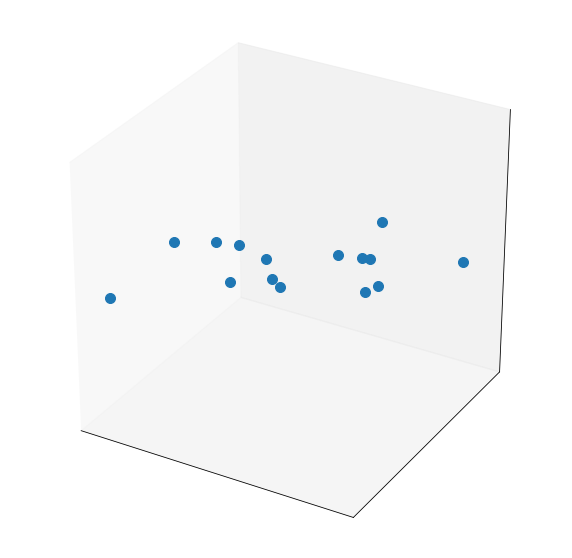
\includegraphics[scale=.4]{Imagenes/search1.png}}
\subfigure[Relaciones inducidas por los operadores de cambio]{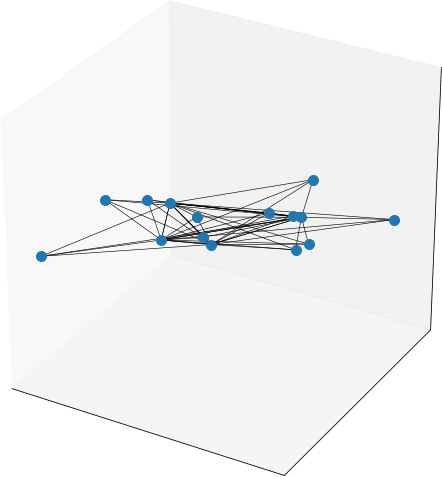
\includegraphics[scale=.4]{Imagenes/search2.png}}
\subfigure[Adición de la función de fitness]{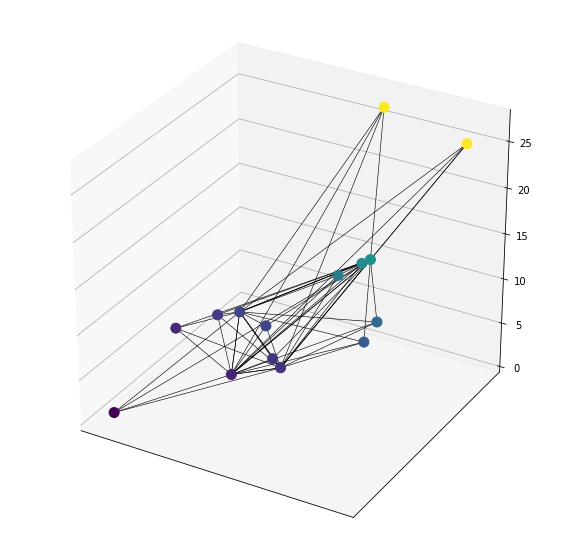
\includegraphics[scale=.4]{Imagenes/search3.png}}
\caption{Creación del paisaje de búsqueda}
\end{figure}
